%%This is a very basic article template.
%%There is just one section and two subsections.
\documentclass[a4paper]{article}
\usepackage{amssymb}
\usepackage{amsmath}
\usepackage{graphicx}
\usepackage{subfigure}
\usepackage{soul}
\usepackage{color}

% soul highlighting config
\setul{1ex}{0.8ex}
\definecolor{orange}{rgb}{1,0.5,0}
\setulcolor{orange}


\begin{document}
	\begin{titlepage}
	
	\centering
	
	{\huge\bfseries Management Dashboard with IBM Cognos\par}
	\vspace{2cm}
	
	
	\begin{figure}
    \subfigure{
\includegraphics[width=0.25\textwidth]{FH}\par\vspace{1cm}}
    \hspace{5cm}
    \subfigure{
\includegraphics[width=0.25\textwidth]{KABEG}\par\vspace{1cm}}
	\end{figure}
	\vspace{1.5cm}
	
	{\Large\itshape Christopher Schmidt\\
	Fabian Matschitsch\par}
	\vfill
	supervised by\par
	Dr.~Florian Hollomey\\
	Dipl. Ing. Gerhard Orlitsch
	\vfill
	{\large \today\par}	
	
	\end{titlepage}

	\tableofcontents
	\newpage

	\section{Introduction}
	Hier wird die Einführung stehen.
	\newpage
	
	\section{Hospital Information Communication}
	\subsection{General Communication}
		The general communication for hospital information is about data of patients,
		medical results, laboratory results, radiographs, financial data, insurance
		data and much more. In the middle of the whole communication will be the
		Hospital Information System (HIS). This system stores the patient information
		and send this data to all other so called Subsystems. A Subsystem will be
		every system which get data from HIS. This systems can also send data back to
		the HIS. For all this communication between the systems there will be a
		standardized protocoll named Health Line 7 (HL7).\\
		The following systems could be subsystems of the Hospital Information System:
		\begin{itemize}
	    	\item Laboratory Information System (LIS)
	    	\item Electronic Medical Record (EMR)
	    	\item Pharmacy Management (PM)
	    	\item Insurance Management (IM)
	    	\item Financial System (FS)
	    	\item Radiology Information System (RIS)
	    	\item Appointment Management (AM)
	    	\item Emergency Management System (EMS)
	    \end{itemize}
	    \begin{figure}[!ht]
		  \centering
		      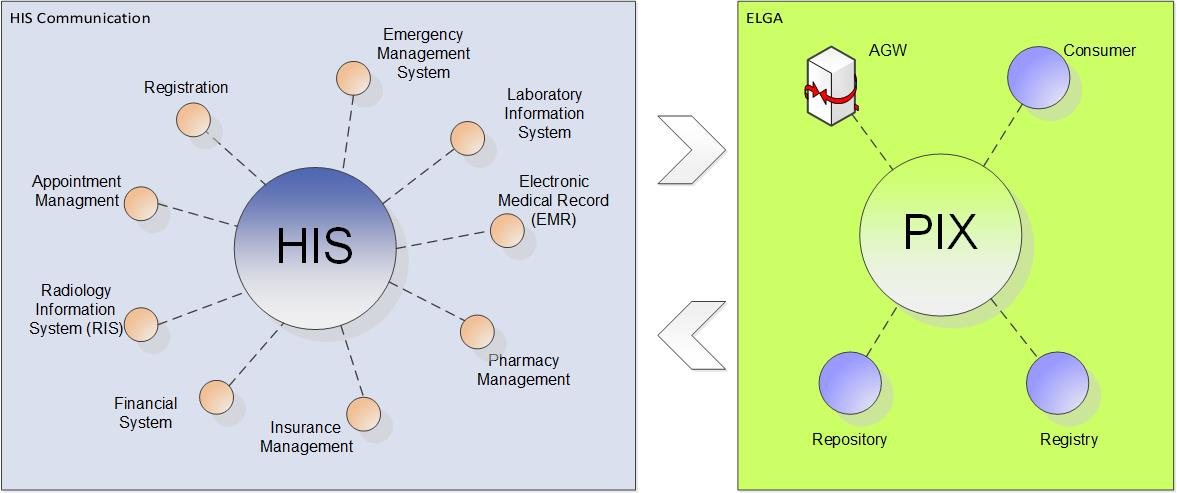
\includegraphics[width=1.0\textwidth]{HIS_Overview}
		  \caption{In the blue box on the left the Hospital Information System
		  Communication is shown. All this system communicate with the ELGA system
		  (on the right) which has an Patient Identifier Cross Referencing (PIX) and
		  an Access Gateway (AGW) for connecting and communicating with external
		  partners.}
		\end{figure}
	    Specially in Austria there will be new kind of system the so called
	    Elektronische Gesundheitsakte (ELGA).
	    This will give the posibility for people in Austria to have a look on their
	    own clinical record in digital way. ELGA and it�s architecture will be explained later on in chapter 4.\\
	    To get the systems speaking together a communcation server will be used.
	    This Server connects all the systems together and it is be able to make
	    mappings and database queries to get the right data in the right fields if
	    they are not.
	\subsection{Health Line 7}
		The Health Line 7 (HL7) is a standardized protocol in Version 2.5 and in
		future in Version 3 for the communication in eHealth systems. All systems
		who were communcating in an hospital will be called eHealth systems.\\
		HL7 provides a framework to exchange, integration, sharing and retrieval of
		electronix health information. It defines also the language, structure and the
		data types which are used for the communicatoin between the eHealth systems.\\
		The standard is human-readable and near to all eHealth systems are able to
		read data from HL7 and to export data in HL7.
		
	\newpage
	
	\section{IBM Cognos Business Intelligence}
	IBM Cognos Business Intelligence (BI) is a software suit designed to extract corporate data from data sources,
	whereby a data source is everything from which persistent information could be retrieved. The extracted data
	can be assembled in the Framework Manager environment to build a so called data warehouse. This warehouse forms
	a foundation from which reports could be created and executed in Report Studio. After reports are created Business
	user could run HTML-based Reports in Cognos Webview. Also automation processes and application of user policies,
	restricting access to reports, can be used.
	
	\subsection{Framework Manager}
	The Framework Manager allows the construction of a logic layer, uniting different data sources in terms of 'query
	items', which grant the possiblity of defining customised queries over, for example, multiple tables in one single
	logical item. Also filtering of the retrieved data can be done.
	\subsubsection{Defining Data Sources}
	Before data can be gathered in Framework Manager, database connections have to be made avialable
	for the Cognos application. Since Cognos is running on a windows server, a driver has to be installed for each type
	of database. This can be done in 'ODBC Data Source Administrator'-Tool. When arranging a connection for the first time,
	the appropriate data source type for the connection has to be chosen. This could be ODBC, ANSI or mixed type for 32- and 64 bit. In
	the figure below an existing figure could be seen:\\
	\begin{figure}[!ht]
		  \centering
		      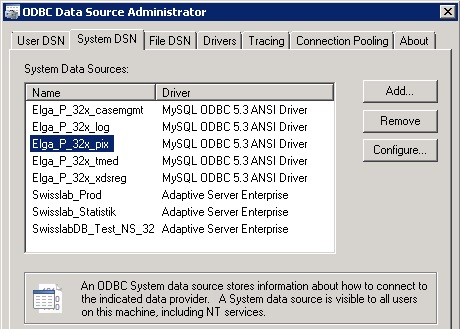
\includegraphics[width=1.0\textwidth]{ExistingDataSource}
		  \caption{}
	\end{figure}
	Furthermore, connection details for the database itself has to be entered for every connection.
	\subsubsection{Frame Manager Surface}
	\hl{Since patient-related Information is used, it must be evaluated how far this information can be revealed.}
	Following figure shows an example of an existing data-warehouse:\\
	\begin{figure}[!ht]
		  \centering
		      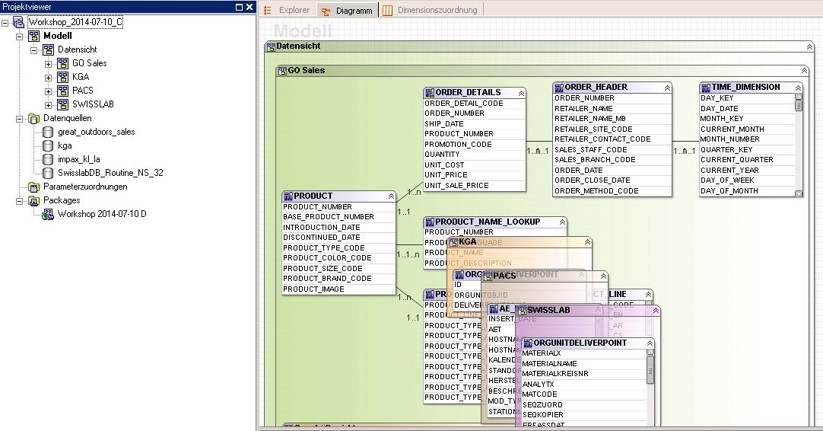
\includegraphics[width=1.0\textwidth]{frameworkM_2}
		  \caption{}
	\end{figure}
	On the left side the project viewer can be seen. It displays in general logical items. This can be data sources,
	views of data sources, which can be modified without altering existing data, and query items. Query items itself
	are highly configurable and allows to define customized and even complex queries. 
	\subsection{Report Studio}
	Overview to Report Studio
	\subsection{Data Topology}
	Overview to Data Topology build in Cognos
	
	\newpage
		
	\section{ELGA }
	In the second quarter of year 2016 ELGA in Carinthia (now on referred as 'ELGA Bereich
	K�rnten' (EBK)) will be connected to central core components. This connection will make
	the availability of documents of citizens and 
	also non-citizens possible in entire Austria. Today, the EBK operates
	as a closed unit which receives data solely from carinthian healthcare providers. 
	At this moment no knowledge about quality, correctness and the total amount of data
	exists, which is mainly needed in decision-making processes.\\
	\\
 	This lack of knowledge should be compensated by the use of IBM Cognos Business 
 	Intelligence, a multi-database environment, by creating a data-warehouse in the KABEG-IT
 	department. A data-warehouse forms a model, consisting of several sources of persistent
 	information, and combines them in a central place.\\
 	\\
	The aim of this project is to build up a prototype-model for the ELGA environment from 
	scratch, using the existing databases. On the basis of this model, HTML-based reports 
	for end-users should be created, which should give the actual amount of patients,
	registered documents (locally and also remote ones), queried documents, number 
	of accesses of users and performance of transactions. When the EBK goes live, a distinction
	between regional-ELGA-relevant documents, also called 'Informationsverbund-documents' (IV)
	and EBK-documents will be made. This distinction will also be integrated in reports.\\
	\\
	
	\subsection{XDS - Cross Document Sharing}
	
	The concept of ELGA, in this case IV and EBK, is described by the term Cross Document Sharing
	(XDS), which allows the exchange of documents between healt care providers, also on federal state level.\\
	This requieres following components:\\
	\begin{itemize}
	    	\item PIX - Patient Identifier Cross-Referencing\\
	    	Each ELGA realm uses its own PIX for managing patients. A central patient index is used to
	    	make cross document sharing possbile.
	    	\item Registry\\
	    	IN general the main task of the registry is to link patients with their related information and also documents.
	    	In detail the jobs and funtions of a registry are much more complex. The will be described in PUNKT DATAMODELL VERLINKEN.
	    	\item Policy Repository\\
	    	Access to documents is managed  by a policy repository. The compliance of patients is entered
	    	by care personal, which can be administration personal for example. For EBK-related this process is similiar, but instead
	    	of using the local repository a central authorization system is used. This allows citizens to manage access to their documents
	    	in general and even after their treatment.
	    	\item XDS Repository\\
	    	A repository which consists of multiple logical formed storages. It saves and provides documents
	    	to healt care providers.
	    	\item XDS Consumer\\
	    	A consumer has the role of a client. It retrieves documents from the XDS repository and displays them for users 
	    	\item AGW - Acces Gateway
	    	Main task of the AGW is to connect the EBK to central components and make Cross Community Access (XCA) between
	    	ELGA realms possible.
	    	\item Radiology Information System (RIS)
	 \end{itemize}
	
	
	
	\subsection{Data Model}
	\hl{Will be written as ELGA goes online, since major changes to the model will be made.
	Since ELGA handels patient-related data, it must be evaluated how far the model can be described.}
	\subsection{Evaluation and Mesurement of Keyfigures}
	\hl{Will be written as ELGA goes online, since major changes to the model will be made.
	Since ELGA handels patient-related data, it must be evaluated how far the Keyfigures can be described.}
	\subsection{Next Steps}
	Next project steps are the finalization of the prototype-model and the expansion
	of reports. The finalization concerns the investigation of different data-warehouse
	schemes in the aspects of time-efficiency and stress-minimization of the running system.
	The reports will be supplemented with a fraud detection-report, which is supposed to 
	give information about unpermitted- and unregularly access of users. Furthermore,
	several fraud detection techniques will be investigated. As EBK goes online, a major
	update of software and datamodels will be executed, making adaption and changes of the
	existing data-warehouse necessary. On the other hand this can also lead to new possibilities
	for integrating additional information in the data-warehouse.
	
	\newpage
	
	\section{Hospital Information System - AGFA Orbis}
	The Hospital Information System is the central system in inter-clinical
	communication. In this system all patient data will be stored and every booking
	and terms for the patients will be made.\\
	In the KABEG there are five hospitals and two different Hospital Information
	Systems. In future there should be only one HIS in the KABEG organisation. This
	HIS will be AGFA Orbis.
	\subsection{Orbis in the KABEG}
	At the moment 4 of 5 KABEG hospitals use AGFA Orbis as HIS. The main
	functionality of Orbis is to collect all patient data and sent it to all
	subsystems.
	\subsection{Orbis Database}
	\subsection{Actual Problems}
	\subsection{Reports for Orbis}
	

\end{document}
